\documentclass[]{article}

\usepackage[autostyle]{csquotes}

\usepackage{color}
\usepackage[usenames,dvipsnames,svgnames,table]{xcolor}
\usepackage[
    backend=biber,
    citestyle=numeric,
    style = numeric,
    sortlocale=de_DE,
    natbib=true,
    url=false, 
    doi=true,
    eprint=false
]{biblatex}
\appto{\bibsetup}{\raggedright}
\addbibresource{bibliography.bib}
\usepackage{hyperref}
\hypersetup{
	colorlinks=true,
	citecolor = black,
	linkcolor = black,
	urlcolor = black
}
\usepackage[T1]{fontenc}
\usepackage{kpfonts}%  for math 
\usepackage{xgreek}
\usepackage{fontspec}
\setmainfont[Ligatures=TeX]{Linux Libertine O}

% for math
\usepackage{amsmath,amsfonts,amsthm, amssymb} % Math packages
\DeclareMathOperator*{\argmin}{arg\,min}
\usepackage{interval}

\usepackage{graphicx}	
\graphicspath{ {images/} }
\usepackage{float}
%%% Custom headers/footers (fancyhdr package)
\usepackage{fancyhdr}
\pagestyle{fancyplain}
\fancyhead{}											% No page header
\fancyfoot[L]{}											% Empty 
\fancyfoot[C]{}											% Empty
\fancyfoot[R]{\thepage}									% Pagenumbering
\renewcommand{\headrulewidth}{0pt}			% Remove header underlines
\renewcommand{\footrulewidth}{0pt}				% Remove footer underlines
\setlength{\headheight}{13.6pt}

%%% Custom sectioning

\usepackage{sectsty}

\allsectionsfont{\centering \normalfont\scshape}

%%% Equation and float numbering
\numberwithin{equation}{section}		% Equationnumbering: section.eq#
\numberwithin{figure}{section}			% Figurenumbering: section.fig#
\numberwithin{table}{section}				% Tablenumbering: section.tab#
\usepackage{subcaption}
\renewcommand\thesubfigure{\roman{subfigure}}

%%% For plotting
\usepackage{array}
\usepackage{graphicx}
\usepackage{multirow}

\newcommand\MyBox[2]{
	\fbox{\lower0.75cm
		\vbox to 1.7cm{\vfil
			\hbox to 1.7cm{\hfil\parbox{1.4cm}{#1\\#2}\hfil}
			\vfil}%
	}%
}

%%% For tables
\usepackage{array}
\usepackage{booktabs}
\setlength{\heavyrulewidth}{1.5pt}
\setlength{\abovetopsep}{4pt}

\newcommand{\horrule}[1]{\rule{\linewidth}{#1}} 	% Horizontal rule

%%% For glossary
\usepackage{glossaries}
\makeglossaries
\newglossaryentry{hpp}{%
	name={HPP},%
	description={Hyperparameter Prediction}%
}
\newglossaryentry{loocv}{%
	name={loocv},%
	description={leave-one-out validation}%
}
\newglossaryentry{smbo}{%
	name={SMBO},%
	description={Sequential model-based Optimization}%
}
\title{
	%\vspace{-1in} 	
	\usefont{OT1}{bch}{b}{n}
	\normalfont \normalsize \textsc{} \\ 
	\horrule{0.5pt} \\[0.4cm]
	\huge  Εκπαίδευση μοντέλου \\πρόβλεψης υπερπαραμέτρων \\αλγορίθμου knn \\
	\horrule{2pt} \\[0.5cm]
}
\author{
	\normalfont 								\normalsize
	Νησιώτη Ελένη\\[-3pt]		\normalsize
	\today
}
\date{}

\setlength{\parindent}{0pt}
\setlength{\parskip}{0.5\baselineskip}%
%% ##############################
\begin{document}
	\maketitle
    \section{Automl: Ρύθμιση Μοντέλου}
    H ρύθμιση ενός μοντέλου μηχανικής μάθησης συνίσταται στην εύρεση των βέλτιστων υπερπαραμέτρων, διαδικασία που υπόκειται στην κρίση του αναλυτή και εμπειρικά αποδεδειγμένα επηρεάζει την απόδοση του τελικού μοντέλου. Η συνηθέστερη τεχνική, που έχει υιοθετήσει η κοινότητα της μηχανικής μάθησης είναι η αναζήτηση των υπερπαραμέτρων σε ένα προκαθορισμένο πλέγμα και η επιλογή των βέλτιστων με cross-validation. Oι \citet{Bergstra:2011:AHO:2986459.2986743} απέδειξαν ότι αυτή η τεχνική είναι υποδεέστερη της τυχαίας αναζήτησης, καθώς αν και οι υπερπαράμετροι κυμαίνονται σε μεγάλο εύρος, μόνο περιορισμένες τιμές επηρεάζουν τη συμπεριφορά του αλγορίθμου, με αποτέλεσμα να δημιουργούνται υποπεριοχές ενδιαφέροντος πρακτικά μη εντοπίσιμες μόνο με πλεγματική αναζήτηση.

    Η επιστήμη του Automl έχει αναγνωρίσει το στάδιο της ρύθμισης μοντέλου ως επιδεχόμενο αυτοματοποίησης λόγω της σημασίας και της χρονικής και υπολογιστικής απαιτητικότητάς του. Ο κύριος άξονας της βιβλιογραφίας είναι η υιοθέτηση τεχνικών βελτιστοποίησης συναρτήσεων μαύρου κουτιού με προσαρμογή τους στις ιδιαιτερότητες των προβλημάτων μηχανικής μάθησης. Παραδείγματα αυτής της προσπάθειας αποτελούν οι βιβλιοθήκες Hyperopt \citep{hyperopt}, Spearmint \citep{spearmint}, HPOlib \citep{hpolib}, οι οποίες υλοποιούν συναρτήσεις \gls{smbo}, η χρήση γενετικών αλγορίθμων \citep{Hutter:2009:EIM:1569901.1569940} και τεχνικών βασισμένων σε gradient descent \citep{wassenberg}.
    
    Στόχος μας είναι η εύρεση των βέλτιστων υπερπαραμέτρων να γίνεται εξολοκλήρου με ένα μοντέλο πρόβλεψης και όχι με αναζήτηση. Προς αυτό το σκοπό θα εκπαιδευτεί ένα μοντέλο πρόβλεψης της υπερπαραμέτρου k ενός knn με χρήση μετα-χαρακτηριστικών,το οποίο ονομάζουμε \gls{hpp} μοντέλο. Η πιθανή και διαπιστωμένη \citep{Feurer:2014:UMI:3015544.3015549} αδυναμία εκπαίδευσης ενός ικανοποιητικά ακριβούς μοντέλου μπορεί να αντιμετωπιστεί με την πρόβλεψη, αντί για μία τιμής, ενός διαστήματος βέλτιστων υπερπαραμέτρων, προερχόμενου από τα διαστήματα πρόβλεψης (\textit{prediction intervals}) του μοντέλου \gls{hpp}. Στη συνέχεια και με βάση αυτό το διάστημα θα εκπαιδεύεται ένα ensemble mοντέλων με την τεχνική του model selection \citep{Caruana:2004:ESL:1015330.1015432}. Κίνητρα για αυτή την προσπαθεια αποτελούν τόσο η επιτάχυνση της διαδικασίας ρύθμισης ενός μοντέλου όσο και η δημιουργία μετα-γνώσης για τη συνάρτηση μεταξύ βέλτιστων υπερπαραμέτρων και φύσης του προβλήματος (χαρακτηριστικά του σετ δεδομένων και του αλγορίθμου μηχανικής μάθησης).
    
    
    \section{Πειράματα}
    Στόχος των πειραμάτων είναι ο καθορισμός του \gls{hpp} μοντέλου. Στην ενότητα 3 θα αξιολογήσουμε την απόδοση του συστήματος, που χρησιμοποιεί το μοντέλο για τη ρύθμιση ενός knn και εκπαιδεύει ένα ensemle knn μοντέλων.  
    
    \subsection{Προετοιμασία} Για τη διεξαγωγή των πειραμάτων συνέλεξα 124 σετ δεδομένων από διάφορες πηγές: UCI \citep{UCI}, kaggle \citep{kaggle}, openml \citep{openml}, data.world \citep{dataworld}, Relational Dataset Repository \citep{relational}. Πρόκειται για σετ δεδομένων δυαδικής ταξινόμησης με πολύ ετερογενή χαρακτηριστικά (πλήθος και είδος χαρακτηριστικών, πλήθος παραδειγμάτων, τύπος αρχείου, παρουσία και αναπαράσταση άγνωστων τιμών, ισορροπία κλάσης). Η διαδικασία που χρησιμοποιήθηκε για τον καθαρισμό τους, ώστε να υπάρχει μια κοινή διεπαφή για το πείραμα ήταν:
    \begin{itemize}
    	\item μετατροπή αρχείων σε comma-delimited .csv. Τα πηγαία αρχεία βρίσκονταν σε μορφές .csv, .txt, .xlsx, .arff, .mysql και είχαν κωδικοποίηση utf-8 ή utf-16.
    	\item καθορισμός κλάσης. Στη πλειοψηφία των περιπτώσεων η κλάση αναγνωριζόταν χειροκίνητα από την περιγραφή του σετ δεδομένων. Συλλέχθηκαν και σετ δεδομένων που ήταν πολλαπλής ταξινόμησης και παλινδρόμησης. Στην πρώτη περίπτωση έγινε αντιστοίχηση σε δύο ουσιώδεις κλάσεις, ενώ στη δεύτερη βρέθηκε η μέση τιμή της μεταβλητής κλάσης και χρησιμοποιήθηκε ως κατώφλι για το διαχωρισμό των παραδειγμάτων σε δύο κλάσεις.
    	\item αναγνώριση άγνωστων τιμών. Στα αρχεία που περιείχαν άγνωστες τιμές χρησιμοποιούνταν διάφοροι συμβολισμοί ("?", "*", "") οι οποίοι αντικαταστάθηκαν από κενά, ώστε να αναγνωρίζονται από την R ως NAs.  
    	\item αναγνώριση ημερομηνιών. Συγκεντρώθηκαν τα ονόματα των χαρακτηριστικών που αναφέρονταν σε ημερομηνίες, ώστε να διαβαστούν σωστά από την R.
    \end{itemize}
    
    Στη συνέχεια παράχθηκαν τα απαραίτητα μετα-δεδομένα για τα πειράματα. Για κάθε σετ δεδομένων  τα μετα-χαρακτηριστικά υπολογίστηκαν με χρήση του πακέτου mfExtractor (που έγραψα εγώ), ενώ η βέλτιστη παράμετρος k βρέθηκε με χρήση του λογισμικού HPOlib \citep{hpolib}, με τον αλγορίθμο βελτιστοποίησης Tree Parzen Estimator για ένα μοντέλο knn της βιβλιοθήκης caret και πλέγμα αναζήτησης $K = \{\, k \mid 1 \le k \le 10 \,\}$.
    
    Για τα πειράματα επιλογής αλγορίθμου το σετ δεδομένων χωρίστηκε σε 58 σετ δεδομένων για εκπαίδευση του \gls{hpp} μοντέλου και 17 για έλεγχό του, καθώς και τον έλεγχο του τελικού συστήματος.
    
    \subsection{Ανάλυση μεταχαρακτηριστικών}
    Η βιβλιογραφία προσφέρει μια εκτεταμένη λίστα μετα-χαρακτηριστικών που μπορούν να χρησιμοποιηθούν για το χαρακτηρισμό ενός σετ δεδομένων. Oι δημιουργοί του autosklearn αναφέρουν τόσο το σύνολο των μετα-χαρακτηριστικών που δοκίμασαν \citep{Feurer:2014:UMI:3015544.3015549} όσο και την τελική λίστα αυτών που συμπεριλήφθηκαν στο τελικό μοντέλο \citep{autosklearn}. Οι \citet{Reif_meta2-features:} προτείνουν την τεχνική των μετα-μετα-χαρακτηριστικών. Στα πειράματά μας δοκιμάσαμε και τα δύο σετ και καταλήξαμε σε αυτό της ομάδας του autosklearn χωρίς τη χρήση landmarking μετα-χαρακτηριστικών . Καθώς το συγκεκριμένο σύνολο δεν αντιπροσωπεύει τα σετ δεδομένων που αποτελούνται μόνο από κατηγορικά χαρακτηριστικά, στόχος μας είναι αυτό το σύνολο να εμπλουτιστεί ώστε να αντικατοπτρίζει όλα τα πιθανά σετ δεδομένων.
    
    \begin{table}[!htb]
    \begin{center}
    	\begin{tabular}{ |c| } 
    		\hline
    		Μετα-χαρακτηριστικά\\
    		\hline
    		Κλάσμα χαρακτηριστικών για 95$\%$ διακύμανση των PCA \\ 
    		Κυρτότητα πρώτης PCA συνιστώσας   \\ 
        	Ασσυμετρία πρώτης PCA συνιστώσας   \\ 
        	Ελάχιστη ασυμμετρία \\
        	Μέγιστη ασυμμετρία \\
        	Μέση τιμή ασυμμετρίας \\
        	Τυπική απόκλιση ασυμμετρίας \\
        	Ελάχιστη κυρτότητα \\
        	Μέγιστη κυρτότητα \\
        	Μέση τιμή κυρτότητας \\
        	Τυπική απόκλιση κυρτότητας \\        	
    		\hline
    	\end{tabular}    
    \end{center}
    	\caption{Τελική λίστα μετα-χαρακτηριστικών}\label{mfs}
    \end{table}
    Η ανάλυση των μετα-χαρακτηριστικών του Σχήματος \ref{mfs} οδήγησε στα ακόλουθα συμπεράσματα:
    \begin{itemize}
    	\item υπάρχει μια μη-γραμμική συσχέτιση μεταξύ των μετα-χαρακτηριστικών που περιγράφουν όμοιες ιδιότητες της ασυμμετρίας και κυρτότητας (Σχήματα \ref{fig:a}, \ref{fig:b} )
    	\item όλα τα χαρακτηριστικά εκτός από τη Μέση τιμή ασυμμετρίας έχουν ξεκάθαρα μη-συμμετρική κατανομή (Σχήματα \ref{fig:c}, \ref{fig:d} )
    	\item υπάρχουν πολλές εξωκείμενες τιμές ( Σχήματα \ref{fig:e}, \ref{fig:f})
    \end{itemize}
    
    %\cleardoublepage
    \begin{figure}[H] % "[t!]" placement specifier just for this example
    	\begin{subfigure}{0.48\textwidth}
    		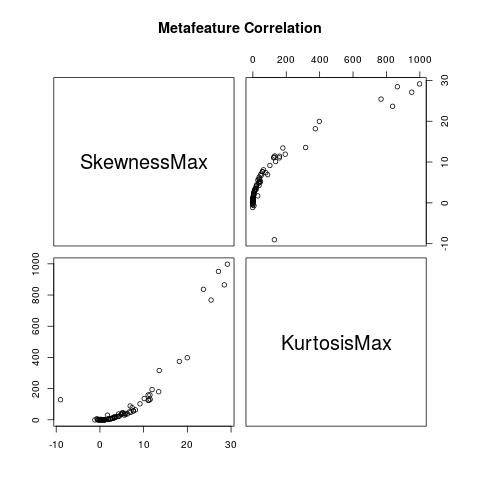
\includegraphics[width=\linewidth, height = 0.2\textheight]{SkewnessMax_KurtosisMax_scatter.jpg}
    		\caption{Λογαριθμική συσχέτιση μεταξύ μέγιστων τιμών κυρτότητας και ασυμμετρίας} \label{fig:a}
    	\end{subfigure}\hspace*{\fill}
    	\begin{subfigure}{0.48\textwidth}
    		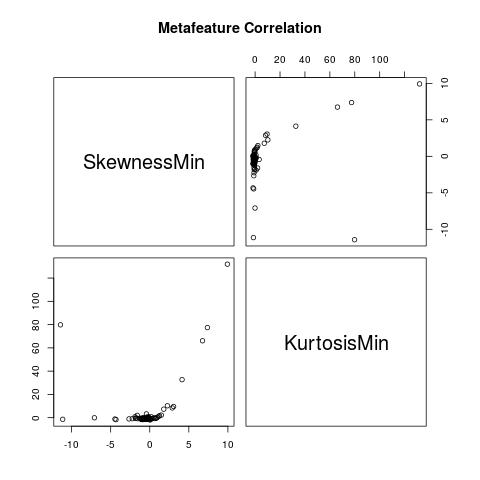
\includegraphics[width=\linewidth, height = 0.2\textheight]{SkewnessMin_KurtosisMin_scatter.jpg}
    		\caption{Λογαριθμική συσχέτιση μεταξύ ελάχιστων τιμών κυρτότητας και ασυμμετρίας} \label{fig:b}
    	\end{subfigure}
    	
    	\medskip
    	\begin{subfigure}{0.48\textwidth}
    		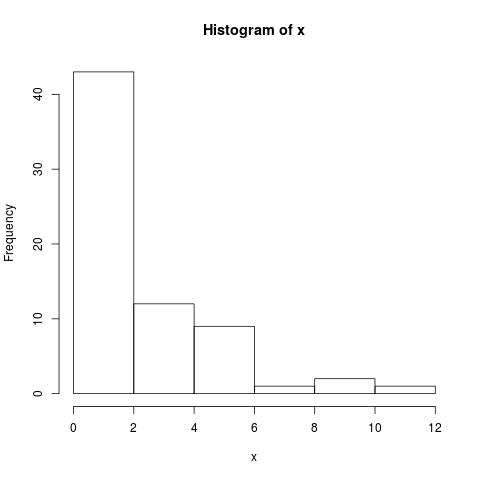
\includegraphics[width=\linewidth, height = 0.2\textheight]{SkewnessSTD_scatter.jpg}
    		\caption{Θετική ασυμμετρία για την τυπική απόκλιση της ασυμμετρίας, όπως και για τα περισσότερα χαρακτηριστικά } \label{fig:c}
    	\end{subfigure}\hspace*{\fill}
    	\begin{subfigure}{0.48\textwidth}
    		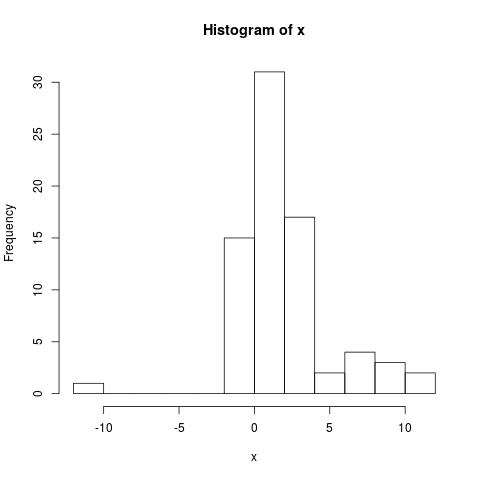
\includegraphics[width=\linewidth, height = 0.2\textheight]{SkewnessMean_scatter.jpg}
    		\caption{Κατανομή κοντινή σε κανονική για τη μέση τιμή της ασυμμετρίας} \label{fig:d}
    	\end{subfigure}
    	
    	\medskip
    	\begin{subfigure}{0.48\textwidth}
    		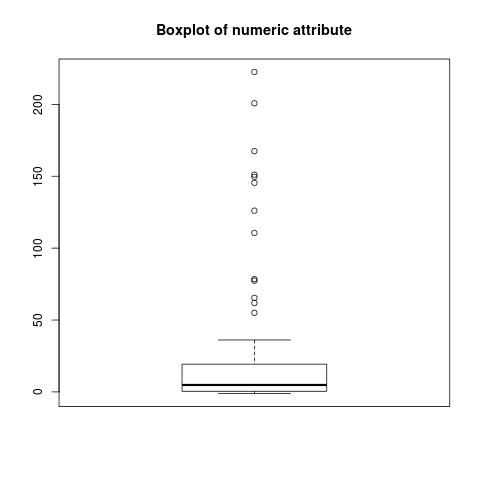
\includegraphics[width=\linewidth, height = 0.2\textheight]{KurtosisMean_boxplot.jpg}
    		\caption{Εμφάνιση πολλών εξωκείμενων τιμών για τη μέση τιμή της κυρτότητας} \label{fig:e}
    	\end{subfigure}\hspace*{\fill}
    	\begin{subfigure}{0.48\textwidth}
    		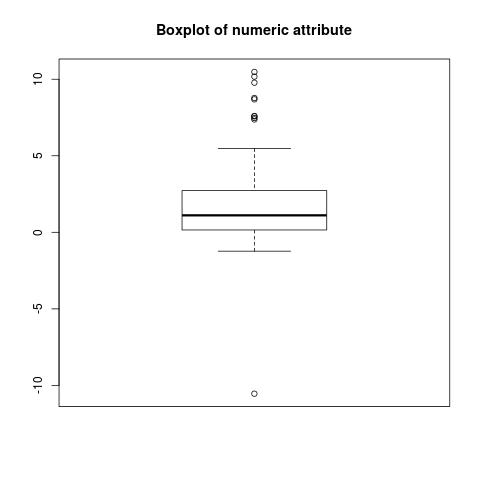
\includegraphics[width=\linewidth, height = 0.2\textheight]{SkewnessMean_boxplot.jpg}
    		\caption{Η κανονική κατανομή της μέσης τιμής της ασσυμετρίας παρουσιάζει επίσης εξωκείμενες τιμές} \label{fig:f}
    	\end{subfigure}
    	
    	\caption{Οπτικοποίηση μετα-χαρακτηριστικών} \label{fig:1}
    \end{figure}
    
    \subsection{Επιλογή αλγορίθμου}    
    
    Αρχικά εξετάστηκε η γραμμικότητα του προβλήματος με χρήση του μοντέλου lm της caret. Κατά την εκπαίδευση ενός μοντέλου παλινδρόμησης υπάρχει η απαίτηση κανονικής κατανομής και σταθερής διακύμανσης των residuals. Σε αντίθετη περίπτωση η χρήση των prediction intervals δεν είναι ορθή. Για να αντιμετωπιστεί αυτό χρησιμοποιούνται μετασχηματισμοί δύναμης, ένας εκ των οποίων είναι ο μετασχηματισμός Box-Cox. Εισήχθη από τους \citet{10.2307/2984418} και ορίζεται ως
    
    \begin{equation}
    y^{'}=
    \begin{cases}
    \frac{y^{\lambda} -1}{\lambda} &  \lambda \neq 0\\
    \log{y} & \lambda = 0
    \end{cases}
    \end{equation} 
    
    Ο μετασχηματισμός αυτός μετατρέπει skewed κατανομές σε κανονικές και κατ' επέκταση εξασφαλίζει γραμμικότητα των χαρακτηριστικών με τη κλάση. Το βέλτιστο $\lambda$ για ένα σετ δεδομένων υπολογίζεται με χρήση profile likelihood διαγραμμάτων, δηλαδή επιλέγεται το $\lambda$ που μεγιστοποιεί την πιθανότητα τα residuals να έχουν κανονική κατανομή με την εφαρμογή του μετασχηματισμού.
    
    Επίσης, εξετάστηκε η χρήση ενός svm, προκειμένου να διαπιστωθεί η αναγκαιότητα ενός πολυπλοκότερου μοντέλου από το γραμμικό. Χρησιμοποιήθηκε το μοντέλο RadialSvm της βιβλιοθήκης caret.
    
   \subsection{Περιγραφή ensemble} Καθώς η απαίτηση ακριβούς πρόβλεψης της βέλτιστης τιμής μιας υπερπαραμέτρου κρίνεται, τουλάχιστον με τα τρέχοντα χαρακτηριστικά, υπερβολικά απαιτητική, όπως σχολίασαν και οι \citet{Feurer:2014:UMI:3015544.3015549}, οι οποίοι αρκέστηκαν στη χρήση των προβλέψεων τους για warmstart αλγορίθμων βελτιστοποίησης, θα χρειαστεί περαιτέρω επεξεργασία του μοντέλου. Προς αυτό το σκοπό εκμεταλλεύτηκα τα διαστήματα πρόβλεψης που παράγονται από ένα γραμμικό μοντέλο και είναι προσβάσιμα μέσω της \textit{caret}, ώστε να ορίσω ένα σύνολο βέλτιστων k για κάθε σετ δεδομένων και να δημιουργήσω έναν ensemble με αυτά. Το σύνολο αυτό ορίζεται ως τα ακέραια k που βρίσκονται στο $90\%$ διάστημα εμπιστοσύνης της πρόβλεψης. Αν η βέλτιστη τιμή βρίσκεται μέσα σε αυτό το διάστημα τότε με χρήση του ensemble θεωρητικά θα εξασφαλιστεί αποτέλεσμα ισάξιο με ένα μοντέλο που θα προέβλεπε επακριβώς τη βέλτιστη υπερπαράμετρο. 
   
   Για τον svm η εξαγωγή των prediction intervals δεν είναι αυτοματοποιημένη. Η τεχνική που ακολουθήθηκε ήταν η εξής: υπολογισμός της διακύμανσης των residuals, εύρεση του e 90$\%$ ποσοστημορίου μιας κανονικής κατανομής με μέση τιμή $\mu$ τις προβλέψεις του μοντέλου και διακύμανση ίση με των residuals και δημιουργία του διαστήματος ως $ \interval{\mu - e}{\mu + e}$
   
   \subsection{Αποτελέσματα}
   \subsubsection{Επιλογή βέλτιστου μοντέλου \gls{hpp}}
   Για την εύρεση του καλύτερου αλγορίθμου χρησιμοποιήθηκαν στατιστικά τεστ. Συγκεκριμένα σύγκρινα τα σφάλματα μεταξύ των μοντέλων \textit{lm} με μετασχηματισμό Βox-Cox, \textit{RadialSvm} και του βελτιστοποιημένου μοντέλου που παρήχθηκε από την \textit{HPOlib} στο 20$\%$ των σετ δεδομένων με χρήση του paired Wilcoxon-rank-sum τεστ σε επίπεδο εμπιστοσύνης $95\%$ για την παρατήρηση στατιστικά σημαντικών διαφορών. Ως σφάλμα ορίζω $e = 1 - accuracy$
   
   \begin{table}[!htb]
   	\begin{center}
   		\begin{tabular}{*5c}
   			\toprule
   			\multicolumn{2}{c}{Μέθοδοι} & \multicolumn{3}{c}{Υπόθεση} \\ 
   			\midrule
   			Μέθοδος 1 & Μέθοδος 2 & Δίπλευρη & Αριστερή & Δεξία\\
   			\midrule
   			svm & HPOlib & 0.0673 & 0.971 & 0.0381 \\
   			lm + BoxCox & HPOlib & 0.1353 & 0.9406 & 0.0673 \\
   			svm & lm + BoxCox & 0.09058 & 0.9608 & 0.04529 \\
   			\midrule   				
   		\end{tabular}    
   	\end{center}
   	\caption{Στατιστική σύγκριση μεθόδων}\label{mfs}
   \end{table}
   
   Με βάση τα παραπάνω στοιχεία συμπεραίνω πως:
   \begin{itemize}
   	\item Δεν μπορώ να απορρίψω την υπόθεση της μηδενικής διαφοράς μεταξύ οποιοδήποτε μεθόδων.
   	\item Μπορώ οριακά να απορρίψω τη μονόπλευρη υπόθεση ότι το μοντέλο svm έχει μεγαλύτερο σφάλμα από το βέλτιστο.
   	\item Επίσης οριακά απορρίπτω την υπόθεση ότι το μοντέλο svm έχει μεγαλύτερο σφάλμα από το μοντέλο lm.
   \end{itemize}
   
   Για τα τελικά πειράματα θα επιλέξω το μοντέλο με μετασχηματισμό Box-Cox, καθώς παρουσιάζει οριακά χειρότερη συμπεριφορά από το svm, αλλά είναι απλούστερο.
   
     
   \subsubsection{Αξιολόγηση \gls{hpp} μοντέλου}
   
   Στη συνέχεια αξιολογούμε την απόδοση του \gls{hpp} μοντέλου. Η ρίζα του μέσου τετραγωνικού σφάλματος, υπολογισμένη με \gls{loocv} είναι 2.56. Στα σχήματα φαίνεται ότι τα residuals του τελικού μοντέλου ακολουθούν σχετικά κανονική κατανομή, επομένως η χρήση των prediction intervals είναι έγκυρη.
   
   \begin{figure}[!htb]
   	\centering
   	\begin{minipage}{.5\textwidth}
   		\centering
   		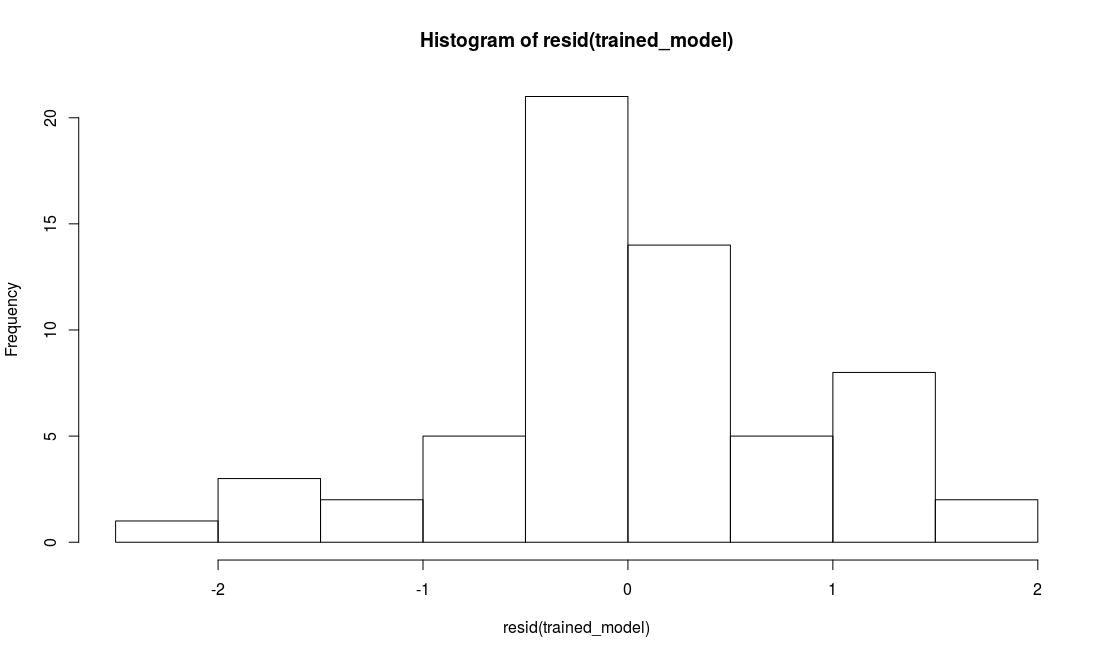
\includegraphics[width=\linewidth, height=0.2\textheight]{hist_resid}
   		\caption{Ιστόγραμμα residuals}
   		\label{fig:1}
   	\end{minipage}%
   	\begin{minipage}{0.5\textwidth}
   		\centering
   		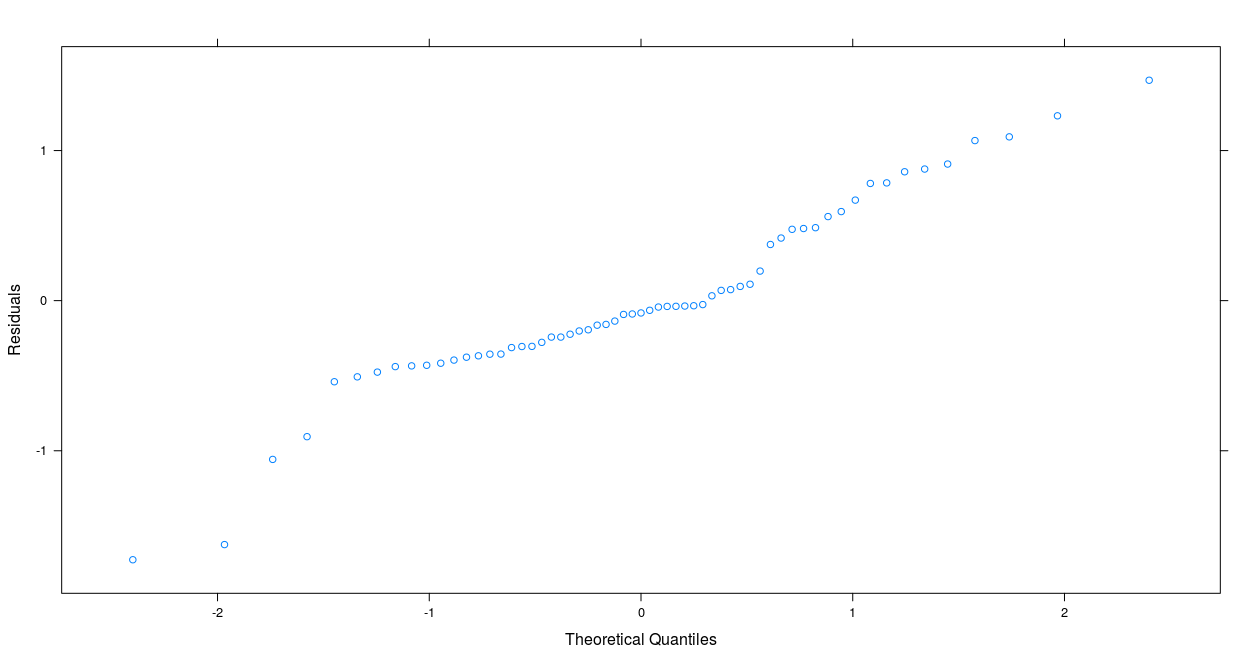
\includegraphics[width=\linewidth, height=0.2\textheight]{lm_trans_resid_qq}
   		\caption{Q-Q διάγραμμα}
   		\label{fig: 2}
   	\end{minipage}
   \end{figure}
   
   Εφαρμόζωντας την τεχνική με τα prediction intervals στο σετ ελέγχου παρατηρούμε ότι πάντα συμπεριλαμβάνουμε τη βέλτιστη λύση
   \begin{figure}
   	\centering
   	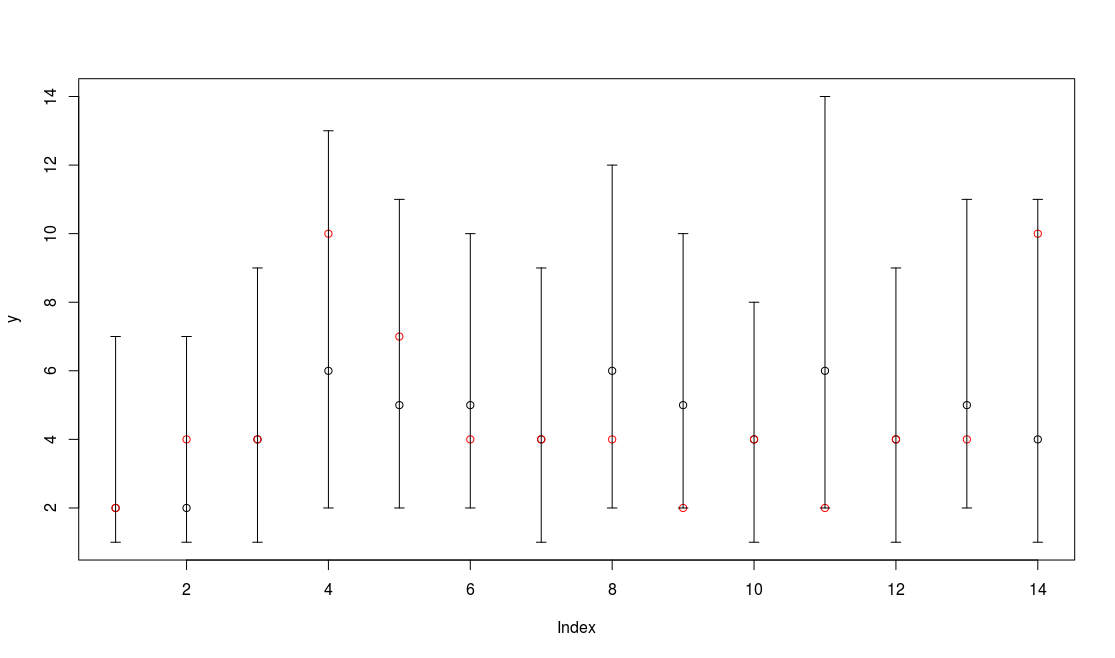
\includegraphics[width=\linewidth, height=0.15\textheight]{intervals}
   	\caption{Διάγραμμα διασποράς προβλέψεων με prediction intervals }
   	\label{fig:1}
   \end{figure}%
   \section{Προτεινόμενο σύστημα}
  	Έχοντας εκπαιδεύσει το \gls{hpp} μοντέλο, θα αξιολογήσουμε το σύστημά μας για τα 17 σετ δεδομένων ελέγχου. Για το καθένα το σύστημα εξάγει τα μετα-χαρακτηριστικά, προβλέπει τα βέλτιστα k με χρήση του \gls{hpp} μοντέλου και σχηματίζει τον ensemble με την τεχνική του model selection. Η απόδοση του ensemble αξιολογείται ως η ακρίβεια με την τεχνική $80\% - 20\%$ holdout.
  	
  	Διαθέτοντας την επιτευχθείσα ακρίβεια και τις ακρίβειες που είχε πετύχει η HPOlib κατά τη βελτιστοποίηση των υπερπαραμέτρων μπορούμε να ερευνήσουμε αν οι δύο μέθοδοι έχουν σημαντική στατιστική διαφορά. Προς αυτό το σκοπό εφαρμόζουμε το paired Wilcoxon-rank-sum τεστ με επίπεδο εμπιστοσύνης $95\%$, σύμφωνα με το οποίο η υπόθεση ότι το προτεινόμενο σύστημα έχει χαμηλότερη ακρίβεια απορρίπτεται με p-value $0.02864$.
   	
 
   	Τα διαγράμματα προφίλ απόδοσης (performance profile plots) \citep{Dolan2002} αποτελούν ένα εργαλείο αξιολόγησης και σύγκρισης της απόδοσης εργαλείων βελτιστοποίησης. Χρησιμοποιούνται σε περιπτώσεις εφαρμογής διαφορετικών τεχνικών βελτιστοποίησης σε ένα σύνολο προβλημάτων ως εναλλακτική απεικόνιση εκτενών πινάκων, μιας συνηθισμένης και προβληματικής λύσης. Το προφίλ απόδοσης είναι η αθροιστική συνάρτηση κατανομής μιας τεχνικής για μία μετρική απόδοσης.
   	
    Ως μετρική απόδοσης ορίζουμε το λόγο της απόδοσης της τρέχουσας τεχνικής προς τη μεγαλύτερη απόδοση που επιτεύχθηκε από οποιαδήποτε τεχνική για ένα συγκεκριμένο σετ δεδομένων, δηλαδή
    
    \begin{equation}
    r_{p,s}= \frac{t_{p,s}}{\max\{{t_{p,s} : s \in S}}\}    
    \end{equation} 
    
    όπου r ο λόγος απόδοσης, t η ακρίβεια, p το σετ δεδομένων και s η τεχνική.
    
    Το διάγραμμα απεικονίζει τη τιμή
     \begin{equation}
     \rho_{\tau}= \frac{size\{{p \in P : r_{p,s} \leq \tau  }\}}{n_p}   
     \end{equation}
      
     η οποία εκφράζει την πιθανότητα μία τεχνική να βρίσκεται σε απόσταση $\tau$ από τον καλύτερο λόγο απόδοσης.  Επομένως το σημείο $\tau = 1$ εκφράζει τη πιθανότητα μία τεχνική να είναι η βέλτιστη.
      
   	Από το διάγραμμα προφίλ απόδοσης που ακολουθεί μπορούμε να συμπεραίνουμε πως το δικό μας μοντέλο είναι πιθανότερα το βέλτιστο. 
   	
   	\begin{figure}[H]
   		\centering
   		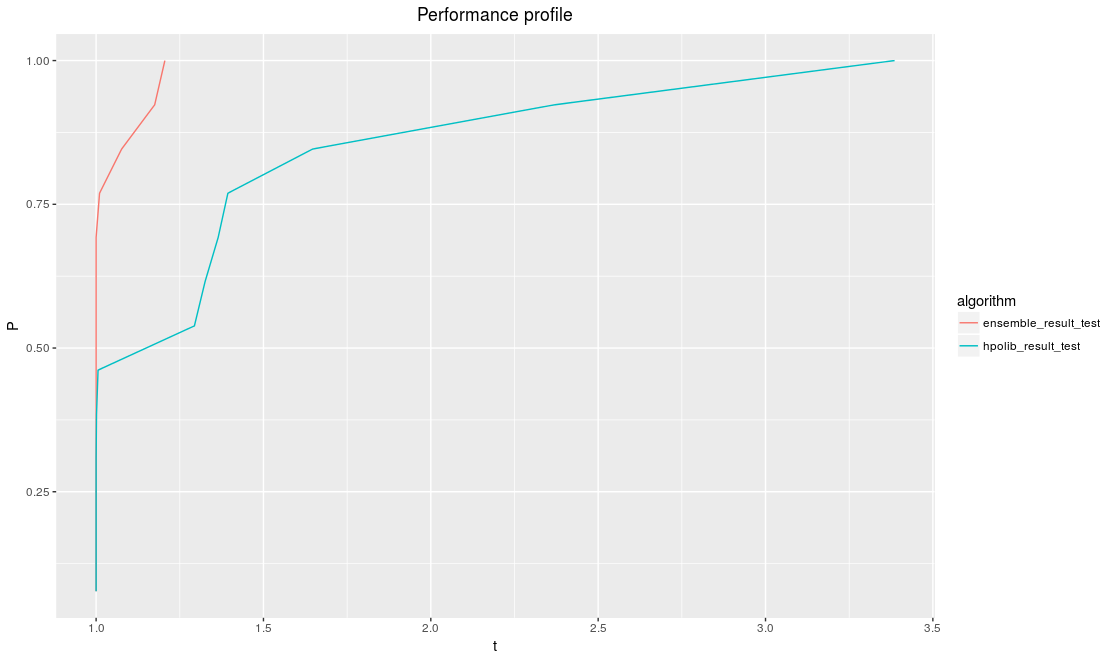
\includegraphics[width=\linewidth, height=0.3\textheight]{perf_prof}
   		\caption{Διάγραμμα απόδοσης για σύγκριση χρήσης προτεινόμενου μοντέλου με βελτιστοποιημένου HPOlib}
   		\label{fig:1}
   	\end{figure}%
   	
   	
    \printbibliography[title= Βιβλιογραφία]
    
    \printglossary[style=long]
\end{document}